% Options for packages loaded elsewhere
\PassOptionsToPackage{unicode}{hyperref}
\PassOptionsToPackage{hyphens}{url}
%
\documentclass[
]{article}
\usepackage{amsmath,amssymb}
\usepackage{lmodern}
\usepackage{ifxetex,ifluatex}
\ifnum 0\ifxetex 1\fi\ifluatex 1\fi=0 % if pdftex
  \usepackage[T1]{fontenc}
  \usepackage[utf8]{inputenc}
  \usepackage{textcomp} % provide euro and other symbols
\else % if luatex or xetex
  \usepackage{unicode-math}
  \defaultfontfeatures{Scale=MatchLowercase}
  \defaultfontfeatures[\rmfamily]{Ligatures=TeX,Scale=1}
\fi
% Use upquote if available, for straight quotes in verbatim environments
\IfFileExists{upquote.sty}{\usepackage{upquote}}{}
\IfFileExists{microtype.sty}{% use microtype if available
  \usepackage[]{microtype}
  \UseMicrotypeSet[protrusion]{basicmath} % disable protrusion for tt fonts
}{}
\makeatletter
\@ifundefined{KOMAClassName}{% if non-KOMA class
  \IfFileExists{parskip.sty}{%
    \usepackage{parskip}
  }{% else
    \setlength{\parindent}{0pt}
    \setlength{\parskip}{6pt plus 2pt minus 1pt}}
}{% if KOMA class
  \KOMAoptions{parskip=half}}
\makeatother
\usepackage{xcolor}
\IfFileExists{xurl.sty}{\usepackage{xurl}}{} % add URL line breaks if available
\IfFileExists{bookmark.sty}{\usepackage{bookmark}}{\usepackage{hyperref}}
\hypersetup{
  pdftitle={Analysis of Activity from a Personal Activity Device},
  hidelinks,
  pdfcreator={LaTeX via pandoc}}
\urlstyle{same} % disable monospaced font for URLs
\usepackage[margin=1in]{geometry}
\usepackage{color}
\usepackage{fancyvrb}
\newcommand{\VerbBar}{|}
\newcommand{\VERB}{\Verb[commandchars=\\\{\}]}
\DefineVerbatimEnvironment{Highlighting}{Verbatim}{commandchars=\\\{\}}
% Add ',fontsize=\small' for more characters per line
\usepackage{framed}
\definecolor{shadecolor}{RGB}{248,248,248}
\newenvironment{Shaded}{\begin{snugshade}}{\end{snugshade}}
\newcommand{\AlertTok}[1]{\textcolor[rgb]{0.94,0.16,0.16}{#1}}
\newcommand{\AnnotationTok}[1]{\textcolor[rgb]{0.56,0.35,0.01}{\textbf{\textit{#1}}}}
\newcommand{\AttributeTok}[1]{\textcolor[rgb]{0.77,0.63,0.00}{#1}}
\newcommand{\BaseNTok}[1]{\textcolor[rgb]{0.00,0.00,0.81}{#1}}
\newcommand{\BuiltInTok}[1]{#1}
\newcommand{\CharTok}[1]{\textcolor[rgb]{0.31,0.60,0.02}{#1}}
\newcommand{\CommentTok}[1]{\textcolor[rgb]{0.56,0.35,0.01}{\textit{#1}}}
\newcommand{\CommentVarTok}[1]{\textcolor[rgb]{0.56,0.35,0.01}{\textbf{\textit{#1}}}}
\newcommand{\ConstantTok}[1]{\textcolor[rgb]{0.00,0.00,0.00}{#1}}
\newcommand{\ControlFlowTok}[1]{\textcolor[rgb]{0.13,0.29,0.53}{\textbf{#1}}}
\newcommand{\DataTypeTok}[1]{\textcolor[rgb]{0.13,0.29,0.53}{#1}}
\newcommand{\DecValTok}[1]{\textcolor[rgb]{0.00,0.00,0.81}{#1}}
\newcommand{\DocumentationTok}[1]{\textcolor[rgb]{0.56,0.35,0.01}{\textbf{\textit{#1}}}}
\newcommand{\ErrorTok}[1]{\textcolor[rgb]{0.64,0.00,0.00}{\textbf{#1}}}
\newcommand{\ExtensionTok}[1]{#1}
\newcommand{\FloatTok}[1]{\textcolor[rgb]{0.00,0.00,0.81}{#1}}
\newcommand{\FunctionTok}[1]{\textcolor[rgb]{0.00,0.00,0.00}{#1}}
\newcommand{\ImportTok}[1]{#1}
\newcommand{\InformationTok}[1]{\textcolor[rgb]{0.56,0.35,0.01}{\textbf{\textit{#1}}}}
\newcommand{\KeywordTok}[1]{\textcolor[rgb]{0.13,0.29,0.53}{\textbf{#1}}}
\newcommand{\NormalTok}[1]{#1}
\newcommand{\OperatorTok}[1]{\textcolor[rgb]{0.81,0.36,0.00}{\textbf{#1}}}
\newcommand{\OtherTok}[1]{\textcolor[rgb]{0.56,0.35,0.01}{#1}}
\newcommand{\PreprocessorTok}[1]{\textcolor[rgb]{0.56,0.35,0.01}{\textit{#1}}}
\newcommand{\RegionMarkerTok}[1]{#1}
\newcommand{\SpecialCharTok}[1]{\textcolor[rgb]{0.00,0.00,0.00}{#1}}
\newcommand{\SpecialStringTok}[1]{\textcolor[rgb]{0.31,0.60,0.02}{#1}}
\newcommand{\StringTok}[1]{\textcolor[rgb]{0.31,0.60,0.02}{#1}}
\newcommand{\VariableTok}[1]{\textcolor[rgb]{0.00,0.00,0.00}{#1}}
\newcommand{\VerbatimStringTok}[1]{\textcolor[rgb]{0.31,0.60,0.02}{#1}}
\newcommand{\WarningTok}[1]{\textcolor[rgb]{0.56,0.35,0.01}{\textbf{\textit{#1}}}}
\usepackage{longtable,booktabs,array}
\usepackage{calc} % for calculating minipage widths
% Correct order of tables after \paragraph or \subparagraph
\usepackage{etoolbox}
\makeatletter
\patchcmd\longtable{\par}{\if@noskipsec\mbox{}\fi\par}{}{}
\makeatother
% Allow footnotes in longtable head/foot
\IfFileExists{footnotehyper.sty}{\usepackage{footnotehyper}}{\usepackage{footnote}}
\makesavenoteenv{longtable}
\usepackage{graphicx}
\makeatletter
\def\maxwidth{\ifdim\Gin@nat@width>\linewidth\linewidth\else\Gin@nat@width\fi}
\def\maxheight{\ifdim\Gin@nat@height>\textheight\textheight\else\Gin@nat@height\fi}
\makeatother
% Scale images if necessary, so that they will not overflow the page
% margins by default, and it is still possible to overwrite the defaults
% using explicit options in \includegraphics[width, height, ...]{}
\setkeys{Gin}{width=\maxwidth,height=\maxheight,keepaspectratio}
% Set default figure placement to htbp
\makeatletter
\def\fps@figure{htbp}
\makeatother
\setlength{\emergencystretch}{3em} % prevent overfull lines
\providecommand{\tightlist}{%
  \setlength{\itemsep}{0pt}\setlength{\parskip}{0pt}}
\setcounter{secnumdepth}{-\maxdimen} % remove section numbering
\ifluatex
  \usepackage{selnolig}  % disable illegal ligatures
\fi

\title{Analysis of Activity from a Personal Activity Device}
\author{}
\date{\vspace{-2.5em}}

\begin{document}
\maketitle

\hypertarget{instructions}{%
\subsection{Instructions}\label{instructions}}

It is now possible to collect a large amount of data about personal
movement using activity monitoring devices such as a Fitbit, Nike
Fuelband, or Jawbone Up. These type of devices are part of the
``quantified self'' movement -- a group of enthusiasts who take
measurements about themselves regularly to improve their health, to find
patterns in their behavior, or because they are tech geeks. But these
data remain under-utilized both because the raw data are hard to obtain
and there is a lack of statistical methods and software for processing
and interpreting the data. This assignment makes use of data from a
personal activity monitoring device. This device collects data at 5
minute intervals through out the day. The data consists of two months of
data from an anonymous individual collected during the months of October
and November, 2012 and include the number of steps taken in 5 minute
intervals each day.

This assignment will be described in multiple parts. You will need to
write a report that answers the questions detailed below. Ultimately,
you will need to complete the entire assignment in a single R markdown
document that can be processed by knitr and be transformed into an HTML
file. For the plotting aspects of this assignment, feel free to use any
plotting system in R (i.e., base, lattice, ggplot2)

Fork/clone the
\href{http://github.com/rdpeng/RepData_PeerAssessment1}{GitHub
repository} created for this assignment. You will submit this assignment
by pushing your completed files into your forked repository on GitHub.
The assignment submission will consist of the URL to your GitHub
repository and the SHA-1 commit ID for your repository state. NOTE: The
GitHub repository also contains the dataset for the assignment so you do
not have to download the data separately.

\hypertarget{data}{%
\subsection{DATA}\label{data}}

The data for this assignment can be downloaded from
\href{https://d396qusza40orc.cloudfront.net/repdata\%2Fdata\%2Factivity.zip}{here}

\textbf{The variables included in this dataset are:}

\begin{itemize}
\item
  steps: Number of steps taking in a 5-minute interval (missing values
  are coded as 𝙽𝙰)
\item
  date: The date on which the measurement was taken in YYYY-MM-DD format
\item
  interval: Identifier for the 5-minute interval in which measurement
  was taken
\item
  The dataset is stored in a comma-separated-value (CSV) file and there
  are a total of 17,568 *
\item
  observations in this dataset.
\end{itemize}

\hypertarget{review-criteria}{%
\subsection{Review Criteria}\label{review-criteria}}

\textbf{1.Repo}

\begin{itemize}
\item
  Valid GitHub URL
\item
  At least one commit beyond the original fork
\item
  Valid SHA-1
\item
  SHA-1 corresponds to a specific commit
\end{itemize}

\textbf{2.Commit containing full submission}

\begin{itemize}
\item
  Code for reading in the dataset and/or processing the data
\item
  Histogram of the total number of steps taken each day
\item
  Mean and median number of steps taken each day
\item
  Time series plot of the average number of steps taken
\item
  The 5-minute interval that, on average, contains the maximum number of
  steps
\item
  Code to describe and show a strategy for imputing missing data
\item
  Histogram of the total number of steps taken each day after missing
  values are imputed
\item
  Panel plot comparing the average number of steps taken per 5-minute
  interval across weekdays and weekends
\item
  All of the R code needed to reproduce the results (numbers, plots,
  etc.) in the report
\end{itemize}

\hypertarget{loading-and-preprocessing-the-data}{%
\subsection{Loading and preprocessing the
data}\label{loading-and-preprocessing-the-data}}

\begin{Shaded}
\begin{Highlighting}[]
\FunctionTok{library}\NormalTok{(tidyverse)}
\FunctionTok{library}\NormalTok{(plyr)}
\FunctionTok{library}\NormalTok{(visdat)}
\FunctionTok{library}\NormalTok{(ggthemes)}
\FunctionTok{library}\NormalTok{(skimr)}
\end{Highlighting}
\end{Shaded}

\hypertarget{data-analysis}{%
\subsection{Data Analysis}\label{data-analysis}}

The following code downloads uploads the file, process and transforms
the data. The Lubridate package can also covert dates.

\begin{Shaded}
\begin{Highlighting}[]
\NormalTok{data }\OtherTok{\textless{}{-}} \FunctionTok{read.csv}\NormalTok{(}\StringTok{"activity.csv"}\NormalTok{, }\AttributeTok{stringsAsFactors =} \ConstantTok{FALSE}\NormalTok{)}
\NormalTok{data}\SpecialCharTok{$}\NormalTok{date }\OtherTok{\textless{}{-}} \FunctionTok{as.Date}\NormalTok{(data}\SpecialCharTok{$}\NormalTok{date, }\StringTok{"\%Y{-}\%m{-}\%d"}\NormalTok{)}

\NormalTok{data }\OtherTok{\textless{}{-}} \FunctionTok{as.data.frame}\NormalTok{(data)}
\NormalTok{data1 }\OtherTok{\textless{}{-}}\NormalTok{ data}
\end{Highlighting}
\end{Shaded}

Calculating the total number of steps. (Group\_by can also be used for
this specific task)

\begin{Shaded}
\begin{Highlighting}[]
\NormalTok{Q1 }\OtherTok{\textless{}{-}} \FunctionTok{ddply}\NormalTok{(data, }\StringTok{"date"}\NormalTok{, summarise,}
            \AttributeTok{nsteps =} \FunctionTok{sum}\NormalTok{(steps, }\AttributeTok{na.rm =} \ConstantTok{TRUE}\NormalTok{))}
\end{Highlighting}
\end{Shaded}

Plotting Histogram with ggplot

\begin{Shaded}
\begin{Highlighting}[]
\FunctionTok{ggplot}\NormalTok{(}\AttributeTok{data =}\NormalTok{ Q1, }\FunctionTok{aes}\NormalTok{(}\AttributeTok{x =}\NormalTok{ nsteps)) }\SpecialCharTok{+}
  \FunctionTok{geom\_histogram}\NormalTok{(}\AttributeTok{fill =} \StringTok{"skyblue"}\NormalTok{, }\AttributeTok{col=}\StringTok{"black"}\NormalTok{,}\AttributeTok{bins =} \DecValTok{20}\NormalTok{) }\SpecialCharTok{+}
  \FunctionTok{xlab}\NormalTok{(}\StringTok{"Total Steps Per Day"}\NormalTok{) }\SpecialCharTok{+}
  \FunctionTok{ylab}\NormalTok{(}\StringTok{"Frequency Count"}\NormalTok{) }\SpecialCharTok{+}
  \FunctionTok{ggtitle}\NormalTok{(}\StringTok{"Total Number of Steps"}\NormalTok{)}
\end{Highlighting}
\end{Shaded}

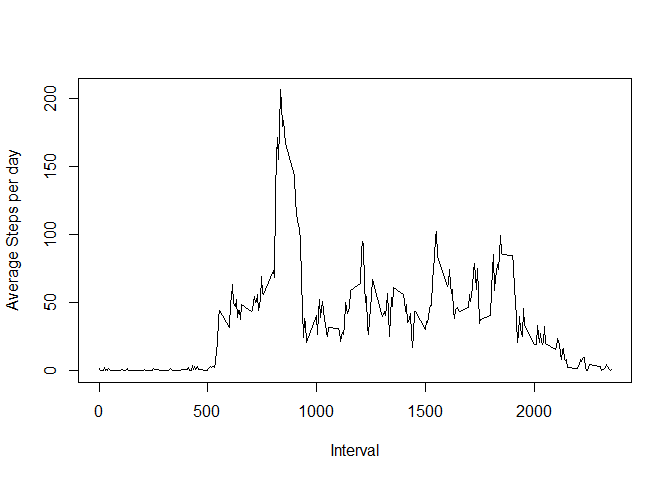
\includegraphics{PA1_EE_files/figure-latex/unnamed-chunk-4-1.pdf}

\hypertarget{what-is-mean-total-number-of-steps-taken-per-day}{%
\subsubsection{What is mean total number of steps taken per
day?}\label{what-is-mean-total-number-of-steps-taken-per-day}}

Calculating the mean and median. Skimr provides a lot of useful
information during data processing.

\begin{Shaded}
\begin{Highlighting}[]
\FunctionTok{skim}\NormalTok{(data)}
\end{Highlighting}
\end{Shaded}

\begin{longtable}[]{@{}ll@{}}
\caption{Data summary}\tabularnewline
\toprule
& \\
\midrule
\endfirsthead
\toprule
& \\
\midrule
\endhead
Name & data \\
Number of rows & 17568 \\
Number of columns & 3 \\
\_\_\_\_\_\_\_\_\_\_\_\_\_\_\_\_\_\_\_\_\_\_\_ & \\
Column type frequency: & \\
Date & 1 \\
numeric & 2 \\
\_\_\_\_\_\_\_\_\_\_\_\_\_\_\_\_\_\_\_\_\_\_\_\_ & \\
Group variables & None \\
\bottomrule
\end{longtable}

\textbf{Variable type: Date}

\begin{longtable}[]{@{}lrrlllr@{}}
\toprule
skim\_variable & n\_missing & complete\_rate & min & max & median &
n\_unique \\
\midrule
\endhead
date & 0 & 1 & 2012-10-01 & 2012-11-30 & 2012-10-31 & 61 \\
\bottomrule
\end{longtable}

\textbf{Variable type: numeric}

\begin{longtable}[]{@{}lrrrrrrrrrl@{}}
\toprule
skim\_variable & n\_missing & complete\_rate & mean & sd & p0 & p25 &
p50 & p75 & p100 & hist \\
\midrule
\endhead
steps & 2304 & 0.87 & 37.38 & 112.00 & 0 & 0.00 & 0.0 & 12.00 & 806 &
▇▁▁▁▁ \\
interval & 0 & 1.00 & 1177.50 & 692.45 & 0 & 588.75 & 1177.5 & 1766.25 &
2355 & ▇▇▇▇▇ \\
\bottomrule
\end{longtable}

\begin{Shaded}
\begin{Highlighting}[]
\FunctionTok{mean}\NormalTok{(Q1}\SpecialCharTok{$}\NormalTok{nsteps)}
\end{Highlighting}
\end{Shaded}

\begin{verbatim}
## [1] 9354.23
\end{verbatim}

\begin{Shaded}
\begin{Highlighting}[]
\FunctionTok{median}\NormalTok{(Q1}\SpecialCharTok{$}\NormalTok{nsteps)}
\end{Highlighting}
\end{Shaded}

\begin{verbatim}
## [1] 10395
\end{verbatim}

\hypertarget{what-is-the-average-daily-activity-pattern}{%
\subsection{What is the average daily activity
pattern?}\label{what-is-the-average-daily-activity-pattern}}

Tapply allows for the means for each interval to be calculated. I would
prefer to use group\_by also works but it seemed to be a be erratic as
is continued with this assignment.

\begin{Shaded}
\begin{Highlighting}[]
\NormalTok{means }\OtherTok{\textless{}{-}} \FunctionTok{with}\NormalTok{(}\FunctionTok{na.omit}\NormalTok{(data), }\FunctionTok{tapply}\NormalTok{(steps, interval, mean))}
\FunctionTok{head}\NormalTok{(means, }\DecValTok{5}\NormalTok{)}
\end{Highlighting}
\end{Shaded}

\begin{verbatim}
##         0         5        10        15        20 
## 1.7169811 0.3396226 0.1320755 0.1509434 0.0754717
\end{verbatim}

\hypertarget{average-daily-activity-pattersn}{%
\subsection{Average daily activity
pattersn}\label{average-daily-activity-pattersn}}

The following code creates a time series plot where y (daily average
steps) per x (5 minute intervals).

\begin{Shaded}
\begin{Highlighting}[]
\NormalTok{Q2 }\OtherTok{\textless{}{-}} \FunctionTok{ddply}\NormalTok{(data, }\StringTok{"interval"}\NormalTok{, summarise,}
            \AttributeTok{nSteps =} \FunctionTok{mean}\NormalTok{(steps, }\AttributeTok{na.rm =} \ConstantTok{TRUE}\NormalTok{))}

\FunctionTok{ggplot}\NormalTok{(}\AttributeTok{data =}\NormalTok{ Q2, }\FunctionTok{aes}\NormalTok{(}\AttributeTok{x=}\NormalTok{ interval, }\AttributeTok{y =}\NormalTok{ nSteps)) }\SpecialCharTok{+}
  \FunctionTok{geom\_line}\NormalTok{(}\AttributeTok{color =} \StringTok{"red"}\NormalTok{) }\SpecialCharTok{+}
  \FunctionTok{xlab}\NormalTok{(}\StringTok{"5 Minute Interval"}\NormalTok{)}\SpecialCharTok{+}
  \FunctionTok{ylab}\NormalTok{(}\StringTok{"Average Steps"}\NormalTok{) }\SpecialCharTok{+}
  \FunctionTok{theme\_economist\_white}\NormalTok{()}
\end{Highlighting}
\end{Shaded}

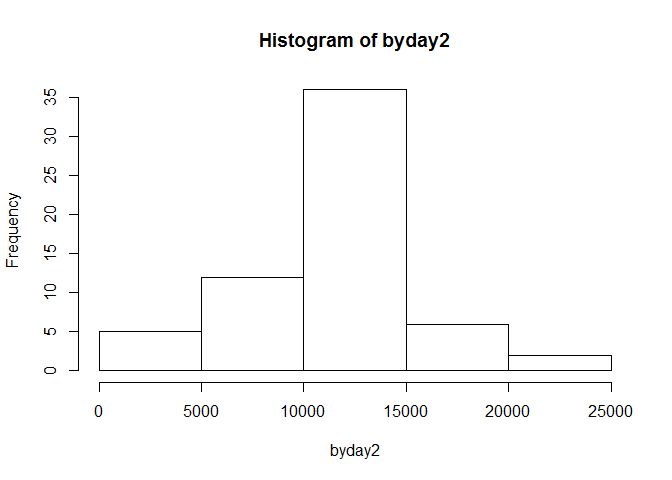
\includegraphics{PA1_EE_files/figure-latex/unnamed-chunk-7-1.pdf}

\begin{Shaded}
\begin{Highlighting}[]
\NormalTok{means[}\FunctionTok{which}\NormalTok{(means }\SpecialCharTok{==} \FunctionTok{max}\NormalTok{(means))]}
\end{Highlighting}
\end{Shaded}

\begin{verbatim}
##      835 
## 206.1698
\end{verbatim}

\hypertarget{imputing-missing-values}{%
\subsection{Imputing missing values}\label{imputing-missing-values}}

Visdat and skimr are helpful in visualizing the type of variable and if
missing data is present.

\begin{Shaded}
\begin{Highlighting}[]
\FunctionTok{sum}\NormalTok{(}\FunctionTok{is.na}\NormalTok{(data))}
\end{Highlighting}
\end{Shaded}

\begin{verbatim}
## [1] 2304
\end{verbatim}

\begin{Shaded}
\begin{Highlighting}[]
\FunctionTok{vis\_dat}\NormalTok{(data)}
\end{Highlighting}
\end{Shaded}

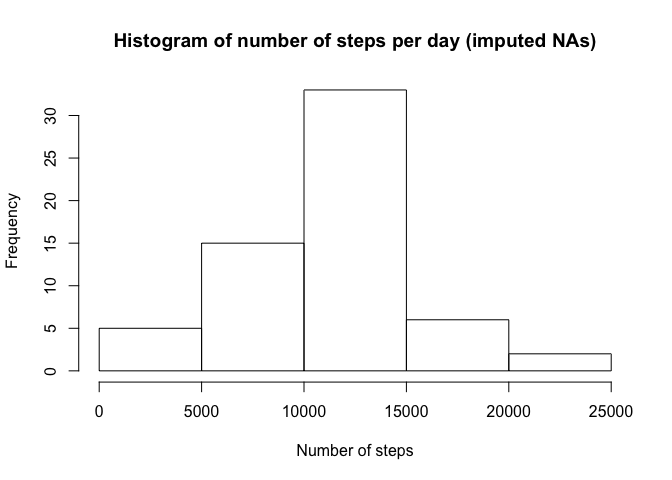
\includegraphics{PA1_EE_files/figure-latex/unnamed-chunk-9-1.pdf}

\begin{Shaded}
\begin{Highlighting}[]
\FunctionTok{vis\_miss}\NormalTok{(data)}
\end{Highlighting}
\end{Shaded}

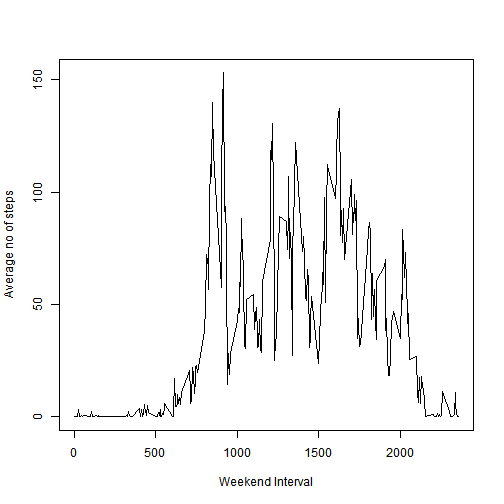
\includegraphics{PA1_EE_files/figure-latex/unnamed-chunk-9-2.pdf}

\begin{Shaded}
\begin{Highlighting}[]
\FunctionTok{skim}\NormalTok{(data)}
\end{Highlighting}
\end{Shaded}

\begin{longtable}[]{@{}ll@{}}
\caption{Data summary}\tabularnewline
\toprule
& \\
\midrule
\endfirsthead
\toprule
& \\
\midrule
\endhead
Name & data \\
Number of rows & 17568 \\
Number of columns & 3 \\
\_\_\_\_\_\_\_\_\_\_\_\_\_\_\_\_\_\_\_\_\_\_\_ & \\
Column type frequency: & \\
Date & 1 \\
numeric & 2 \\
\_\_\_\_\_\_\_\_\_\_\_\_\_\_\_\_\_\_\_\_\_\_\_\_ & \\
Group variables & None \\
\bottomrule
\end{longtable}

\textbf{Variable type: Date}

\begin{longtable}[]{@{}lrrlllr@{}}
\toprule
skim\_variable & n\_missing & complete\_rate & min & max & median &
n\_unique \\
\midrule
\endhead
date & 0 & 1 & 2012-10-01 & 2012-11-30 & 2012-10-31 & 61 \\
\bottomrule
\end{longtable}

\textbf{Variable type: numeric}

\begin{longtable}[]{@{}lrrrrrrrrrl@{}}
\toprule
skim\_variable & n\_missing & complete\_rate & mean & sd & p0 & p25 &
p50 & p75 & p100 & hist \\
\midrule
\endhead
steps & 2304 & 0.87 & 37.38 & 112.00 & 0 & 0.00 & 0.0 & 12.00 & 806 &
▇▁▁▁▁ \\
interval & 0 & 1.00 & 1177.50 & 692.45 & 0 & 588.75 & 1177.5 & 1766.25 &
2355 & ▇▇▇▇▇ \\
\bottomrule
\end{longtable}

\begin{Shaded}
\begin{Highlighting}[]
\FunctionTok{nrow}\NormalTok{(data)}
\end{Highlighting}
\end{Shaded}

\begin{verbatim}
## [1] 17568
\end{verbatim}

\begin{Shaded}
\begin{Highlighting}[]
\NormalTok{(}\DecValTok{2304}\SpecialCharTok{/}\DecValTok{17568}\NormalTok{)}
\end{Highlighting}
\end{Shaded}

\begin{verbatim}
## [1] 0.1311475
\end{verbatim}

\begin{Shaded}
\begin{Highlighting}[]
\FunctionTok{head}\NormalTok{(data)}
\end{Highlighting}
\end{Shaded}

\begin{verbatim}
##   steps       date interval
## 1    NA 2012-10-01        0
## 2    NA 2012-10-01        5
## 3    NA 2012-10-01       10
## 4    NA 2012-10-01       15
## 5    NA 2012-10-01       20
## 6    NA 2012-10-01       25
\end{verbatim}

\begin{Shaded}
\begin{Highlighting}[]
\FunctionTok{tail}\NormalTok{(data)}
\end{Highlighting}
\end{Shaded}

\begin{verbatim}
##       steps       date interval
## 17563    NA 2012-11-30     2330
## 17564    NA 2012-11-30     2335
## 17565    NA 2012-11-30     2340
## 17566    NA 2012-11-30     2345
## 17567    NA 2012-11-30     2350
## 17568    NA 2012-11-30     2355
\end{verbatim}

Made a copy of the data.

\begin{Shaded}
\begin{Highlighting}[]
\NormalTok{data2 }\OtherTok{\textless{}{-}}\NormalTok{ data}
\end{Highlighting}
\end{Shaded}

The following code served the following purposes:

\begin{itemize}
\item
  intUQ: helped in obtaining the number of unique ``interval'' values.
\item
  rows: obtaining the rows of missing data.
\item
  NAintr: number of missing values in ther interval column.
\item
  STEPSna: missing values in the steps column.
\end{itemize}

\begin{Shaded}
\begin{Highlighting}[]
\NormalTok{intUQ }\OtherTok{\textless{}{-}} \FunctionTok{unique}\NormalTok{(data2}\SpecialCharTok{$}\NormalTok{interval)  }
\NormalTok{rows }\OtherTok{\textless{}{-}} \FunctionTok{nrow}\NormalTok{(data[}\FunctionTok{is.na}\NormalTok{(data2), ]) }

\NormalTok{NAintr }\OtherTok{\textless{}{-}}\NormalTok{ data[}\FunctionTok{is.na}\NormalTok{(data2), }\DecValTok{3}\NormalTok{] }
\NormalTok{STEPSna }\OtherTok{\textless{}{-}}\NormalTok{data[}\FunctionTok{is.na}\NormalTok{(data2), }\DecValTok{1}\NormalTok{]  }
\end{Highlighting}
\end{Shaded}

\#\#\#\textbf{Creating a function that deals with missing values.}

Dinov's data science textbook ( 2018:79-81) was usefu in creating a
function that deals with missing values.

\begin{itemize}
\item
  j: for missing row values
\item
  i: for missing interval values
\end{itemize}

\begin{Shaded}
\begin{Highlighting}[]
\ControlFlowTok{for}\NormalTok{ (j }\ControlFlowTok{in} \DecValTok{1}\SpecialCharTok{:}\DecValTok{2304}\NormalTok{)\{       }\CommentTok{\# missing values }
  \ControlFlowTok{for}\NormalTok{ (i }\ControlFlowTok{in} \DecValTok{1}\SpecialCharTok{:}\DecValTok{288}\NormalTok{) \{     }\CommentTok{\# number of intervals }
    \ControlFlowTok{if}\NormalTok{(NAintr[j] }\SpecialCharTok{==}\NormalTok{ intUQ[i]) }\CommentTok{\# if they are equal t}
\NormalTok{      STEPSna[j] }\OtherTok{\textless{}{-}}\NormalTok{ means[i] }\CommentTok{\# then replace with the means from the mneans columns}
\NormalTok{  \}}
\NormalTok{\}}
\end{Highlighting}
\end{Shaded}

\begin{itemize}
\item
  indX: number of missing values from steps
\item
  Missing steps (using indX as an index) are replaced
\end{itemize}

\begin{Shaded}
\begin{Highlighting}[]
\NormalTok{indX }\OtherTok{\textless{}{-}} \FunctionTok{is.na}\NormalTok{(data}\SpecialCharTok{$}\NormalTok{steps)}
\NormalTok{data}\SpecialCharTok{$}\NormalTok{steps }\OtherTok{\textless{}{-}} \FunctionTok{replace}\NormalTok{(data}\SpecialCharTok{$}\NormalTok{steps, indX, STEPSna)}
\FunctionTok{head}\NormalTok{(data)}
\end{Highlighting}
\end{Shaded}

\begin{verbatim}
##       steps       date interval
## 1 1.7169811 2012-10-01        0
## 2 0.3396226 2012-10-01        5
## 3 0.1320755 2012-10-01       10
## 4 0.1509434 2012-10-01       15
## 5 0.0754717 2012-10-01       20
## 6 2.0943396 2012-10-01       25
\end{verbatim}

\begin{itemize}
\tightlist
\item
  Make a histogram of the total number of steps taken each day and
  Calculate and report the mean and median total number of steps taken
  per day. Do these values differ from the estimates from the first part
  of the assignment? What is the impact of imputing missing data on the
  estimates of the total daily number of steps?
\end{itemize}

\begin{Shaded}
\begin{Highlighting}[]
\NormalTok{Q3 }\OtherTok{\textless{}{-}} \FunctionTok{ddply}\NormalTok{(data2, }\StringTok{"date"}\NormalTok{, summarise, }\AttributeTok{Nsteps =} \FunctionTok{sum}\NormalTok{(steps, }\AttributeTok{na.rm =} \ConstantTok{TRUE}\NormalTok{))}

\FunctionTok{ggplot}\NormalTok{(}\AttributeTok{data =}\NormalTok{ Q3, }\FunctionTok{aes}\NormalTok{(}\AttributeTok{x =}\NormalTok{ Nsteps)) }\SpecialCharTok{+}
  \FunctionTok{geom\_histogram}\NormalTok{(}\AttributeTok{fill =} \StringTok{"skyblue"}\NormalTok{, }\AttributeTok{col =} \StringTok{"red"}\NormalTok{, }\AttributeTok{bins =} \DecValTok{20}\NormalTok{) }\SpecialCharTok{+}
  \FunctionTok{xlab}\NormalTok{(}\StringTok{"Total Steps per Day"}\NormalTok{) }\SpecialCharTok{+}
  \FunctionTok{ylab}\NormalTok{(}\StringTok{"Frequency (count)"}\NormalTok{) }\SpecialCharTok{+}
  \FunctionTok{theme\_clean}\NormalTok{()}
\end{Highlighting}
\end{Shaded}

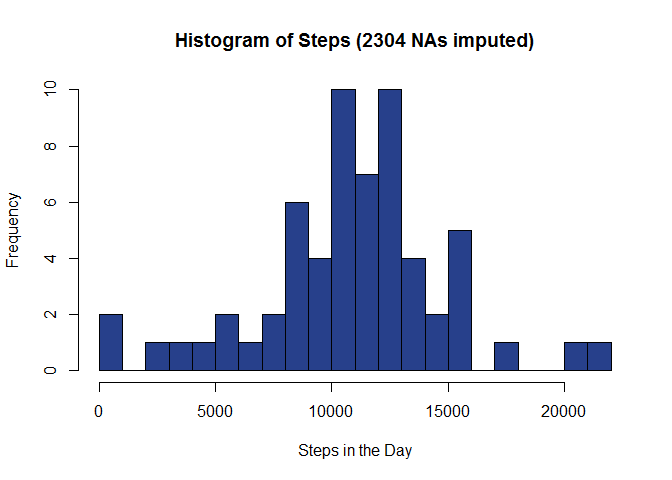
\includegraphics{PA1_EE_files/figure-latex/unnamed-chunk-14-1.pdf}

Do these values differ from the estimates from the first part of the
assignment? What is the impact of imputing missing data on the estimates
of the total daily number of steps?

\begin{itemize}
\tightlist
\item
  Calculated steps taken by day.
\end{itemize}

\begin{Shaded}
\begin{Highlighting}[]
\NormalTok{steps }\OtherTok{\textless{}{-}} \FunctionTok{with}\NormalTok{(}\AttributeTok{data =}\NormalTok{ data, }\FunctionTok{tapply}\NormalTok{(steps,date, sum))}
\FunctionTok{vis\_dat}\NormalTok{(data)}
\end{Highlighting}
\end{Shaded}

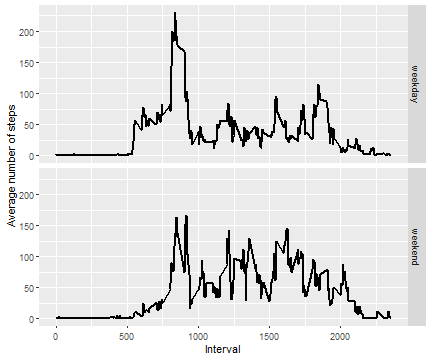
\includegraphics{PA1_EE_files/figure-latex/unnamed-chunk-15-1.pdf}

\begin{Shaded}
\begin{Highlighting}[]
\FunctionTok{vis\_miss}\NormalTok{(data)}
\end{Highlighting}
\end{Shaded}

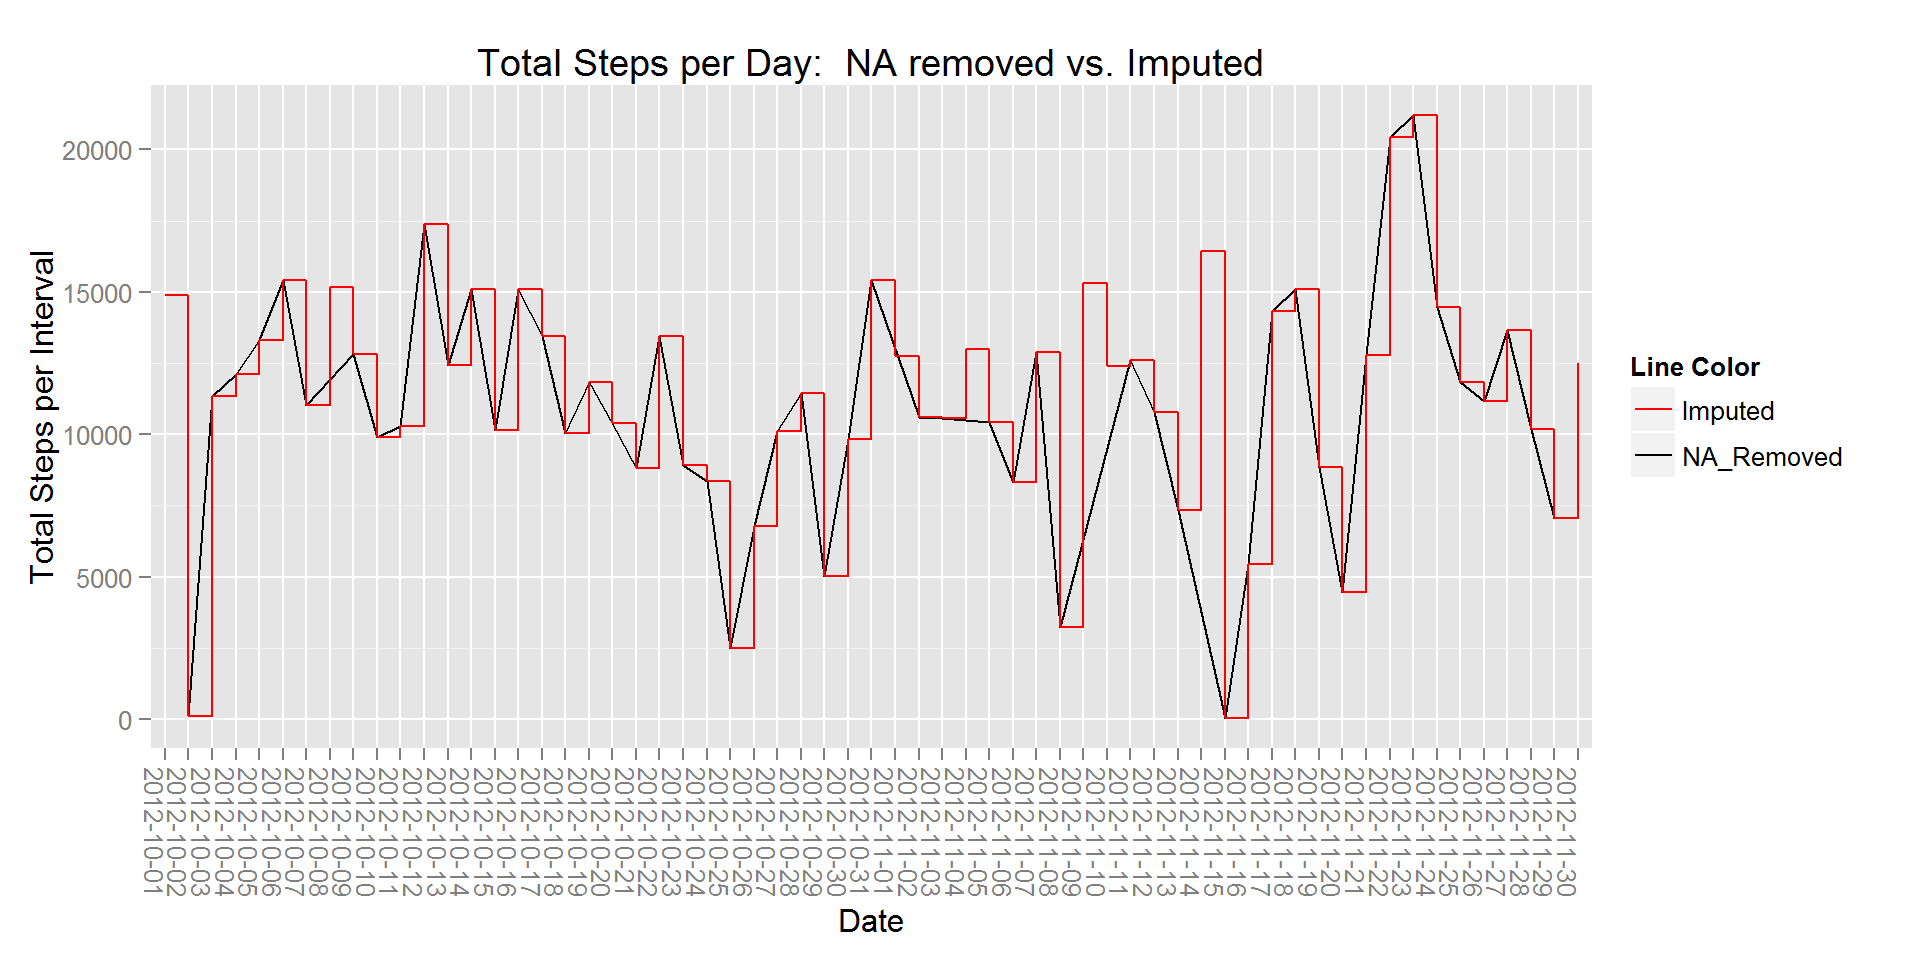
\includegraphics{PA1_EE_files/figure-latex/unnamed-chunk-15-2.pdf}

\begin{Shaded}
\begin{Highlighting}[]
\FunctionTok{mean}\NormalTok{(steps)}
\end{Highlighting}
\end{Shaded}

\begin{verbatim}
## [1] 10766.19
\end{verbatim}

\begin{Shaded}
\begin{Highlighting}[]
\FunctionTok{median}\NormalTok{(steps)}
\end{Highlighting}
\end{Shaded}

\begin{verbatim}
## [1] 10766.19
\end{verbatim}

\textbf{Answer: Yes, the replacement of NA values with interval means.
As a result, the mean and median are similar.}

\hypertarget{are-there-differences-in-activity-patterns-between-weekdays-and-weekends}{%
\subsection{Are there differences in activity patterns between weekdays
and
weekends?}\label{are-there-differences-in-activity-patterns-between-weekdays-and-weekends}}

A copy of the data was created.

\begin{Shaded}
\begin{Highlighting}[]
\NormalTok{Q3 }\OtherTok{\textless{}{-}}\NormalTok{ data}
\NormalTok{Q3 }\OtherTok{\textless{}{-}} \FunctionTok{mutate}\NormalTok{(Q3, }\AttributeTok{day =} \FunctionTok{weekdays}\NormalTok{(Q3}\SpecialCharTok{$}\NormalTok{date))}
\NormalTok{Q3 }\OtherTok{\textless{}{-}} \FunctionTok{as.data.frame}\NormalTok{(Q3)}
\end{Highlighting}
\end{Shaded}

This portion of the assignment requires that a new factor variable
(``day'') be created with two levels differentiating the week: weekend
and weekday.

\begin{Shaded}
\begin{Highlighting}[]
\NormalTok{weekdays }\OtherTok{\textless{}{-}} \FunctionTok{c}\NormalTok{(}\StringTok{\textquotesingle{}Monday\textquotesingle{}}\NormalTok{, }\StringTok{\textquotesingle{}Tuesday\textquotesingle{}}\NormalTok{, }\StringTok{\textquotesingle{}Wednesday\textquotesingle{}}\NormalTok{, }\StringTok{\textquotesingle{}Thursday\textquotesingle{}}\NormalTok{, }\StringTok{\textquotesingle{}Friday\textquotesingle{}}\NormalTok{)}
\NormalTok{Q3}\SpecialCharTok{$}\NormalTok{day }\OtherTok{\textless{}{-}} \FunctionTok{factor}\NormalTok{((}\FunctionTok{weekdays}\NormalTok{(Q3}\SpecialCharTok{$}\NormalTok{date) }\SpecialCharTok{\%in\%}\NormalTok{ weekdays), }
                 \AttributeTok{levels=}\FunctionTok{c}\NormalTok{(}\ConstantTok{FALSE}\NormalTok{, }\ConstantTok{TRUE}\NormalTok{), }\AttributeTok{labels=}\FunctionTok{c}\NormalTok{(}\StringTok{\textquotesingle{}Weekend\textquotesingle{}}\NormalTok{, }\StringTok{\textquotesingle{}Weekday\textquotesingle{}}\NormalTok{))}
\end{Highlighting}
\end{Shaded}

Two subsets of data were created.

\begin{Shaded}
\begin{Highlighting}[]
\NormalTok{weekdays }\OtherTok{\textless{}{-}} \FunctionTok{subset}\NormalTok{(Q3, day }\SpecialCharTok{==} \StringTok{"Weekday"}\NormalTok{)}
\NormalTok{weekends }\OtherTok{\textless{}{-}} \FunctionTok{subset}\NormalTok{(Q3, day }\SpecialCharTok{==} \StringTok{"Weekend"}\NormalTok{)}
\end{Highlighting}
\end{Shaded}

Before calculating the means, two subsets based on day were created.
Although this approach may take a couple of more lines of code, it
helped in following the process taken to answer this question.

\begin{Shaded}
\begin{Highlighting}[]
\NormalTok{wday }\OtherTok{\textless{}{-}} \FunctionTok{aggregate}\NormalTok{(steps}\SpecialCharTok{\textasciitilde{}}\NormalTok{interval, weekdays, mean)}
\NormalTok{wend }\OtherTok{\textless{}{-}} \FunctionTok{aggregate}\NormalTok{(steps}\SpecialCharTok{\textasciitilde{}}\NormalTok{interval, weekends, mean)}
\end{Highlighting}
\end{Shaded}

Merging the two subsets.

\begin{itemize}
\tightlist
\item
  Only the column for means steps during the weekend from the weekend
  subset was included.
\end{itemize}

\begin{Shaded}
\begin{Highlighting}[]
\NormalTok{days\_activity }\OtherTok{\textless{}{-}} \FunctionTok{cbind}\NormalTok{(wday,wend}\SpecialCharTok{$}\NormalTok{steps)}
\end{Highlighting}
\end{Shaded}

Names were changed to reflect weekend and weekday.

\begin{Shaded}
\begin{Highlighting}[]
\FunctionTok{names}\NormalTok{(days\_activity)[}\DecValTok{2}\NormalTok{] }\OtherTok{\textless{}{-}} \StringTok{"Weekday"}
\FunctionTok{names}\NormalTok{(days\_activity)[}\DecValTok{3}\NormalTok{] }\OtherTok{\textless{}{-}} \StringTok{"Weekend"}
\end{Highlighting}
\end{Shaded}

\begin{Shaded}
\begin{Highlighting}[]
\NormalTok{p1 }\OtherTok{\textless{}{-}} \FunctionTok{ggplot}\NormalTok{(}\AttributeTok{data =}\NormalTok{ days\_activity, }\FunctionTok{aes}\NormalTok{(}\AttributeTok{x =}\NormalTok{ interval, }\AttributeTok{y =}\NormalTok{ Weekday, }\AttributeTok{col =} \StringTok{"black"}\NormalTok{)) }\SpecialCharTok{+} 
  \FunctionTok{geom\_line}\NormalTok{() }\SpecialCharTok{+} \FunctionTok{theme\_fivethirtyeight}\NormalTok{() }\SpecialCharTok{+} \FunctionTok{ggtitle}\NormalTok{(}\StringTok{"Avg Daily Activity by Weekdays/Weekend"}\NormalTok{)}
\end{Highlighting}
\end{Shaded}

Patchwork is a ggplot packaged with some added feature. In this case, it
made faceting this graph much easier.

\begin{Shaded}
\begin{Highlighting}[]
\FunctionTok{library}\NormalTok{(patchwork)}
\end{Highlighting}
\end{Shaded}

\begin{Shaded}
\begin{Highlighting}[]
\NormalTok{p2 }\OtherTok{\textless{}{-}} \FunctionTok{ggplot}\NormalTok{(}\AttributeTok{data =}\NormalTok{ days\_activity, }\FunctionTok{aes}\NormalTok{(}\AttributeTok{x =}\NormalTok{ interval, }\AttributeTok{y =}\NormalTok{ Weekend, }\AttributeTok{col =}\StringTok{"red"}\NormalTok{)) }\SpecialCharTok{+} 
  \FunctionTok{geom\_line}\NormalTok{()}\SpecialCharTok{+} \FunctionTok{theme\_fivethirtyeight}\NormalTok{()}
\end{Highlighting}
\end{Shaded}

\begin{Shaded}
\begin{Highlighting}[]
\NormalTok{Final }\OtherTok{\textless{}{-}}\NormalTok{ p1 }\SpecialCharTok{/}\NormalTok{ p2}
\NormalTok{Final }\SpecialCharTok{+} \FunctionTok{xlab}\NormalTok{(}\StringTok{"Interval"}\NormalTok{) }\SpecialCharTok{+} \FunctionTok{ylab}\NormalTok{(}\StringTok{"Number of Steps"}\NormalTok{) }\SpecialCharTok{+}
  \FunctionTok{xlim}\NormalTok{(}\DecValTok{0}\NormalTok{,}\DecValTok{2500}\NormalTok{)}
\end{Highlighting}
\end{Shaded}

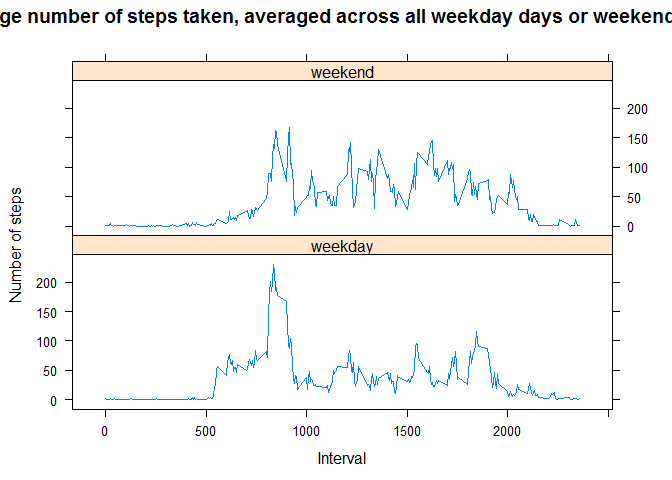
\includegraphics{PA1_EE_files/figure-latex/unnamed-chunk-25-1.pdf}

\begin{itemize}
\tightlist
\item
  Are there differences in activity patterns between weekdays and
  weekends?
\end{itemize}

\textbf{Answer:There is a difference between activity patterns between
weekend and weekdays. Evidence shows there is a decrease in average
steps per day in the weekends.}

\end{document}
